推荐系统(Recommender Systems)是一种信息过滤系统,其研究的目的是让系统预测用户(user)对物品(item)的“评分”或“偏好”。目前推荐系统以其不同的推荐目标,可以划分为序列推荐(Sequential Recommender)、知识图谱推荐(Knowledge-based Recommender)、对话推荐(Conversational Recommender)以及标签感知推荐系统(Tag-aware Recommender)等。本文主要研究范围是标签感知推荐。
\section{研究背景及意义}
随着信息技术和互联网大数据的飞速发展,现代社会已经进入了信息爆炸的时代。在这个信息量急剧上升的时代,各大内容服务平台的数据资源规模呈指数级增长。然而,数据资源在应用的数据平台中大量积累,导致了信息超载(information overload)的问题,这已经成为互联网用户面临的重要挑战之一\cite{cn2022w}。

传统的搜索引擎已经难以为用户提供高效的信息检索服务,用户无法从丰富但相似、庞杂且无序的信息中有效地获取所需的信息。在这种信息超载的大环境下,如何为用户过滤冗余信息,提供独特而精准的个性化推荐服务已经成为了各大内容服务平台的核心业务之一。为此,这些平台相继构建起符合平台业务需求的工业规模推荐系统,基于用户与平台的交互信息,预测用户对数据资源的评分和偏好,从而提供以用户为中心的个性化推荐服务\cite{covington_deep_2016}。

例如,淘宝、京东等电子商务平台\cite{wang_billion-scale_2018}致力于为用户提供感兴趣的商品;抖音、快手等短视频平台\cite{liu_monolith_2022}为用户推送符合偏好的视频;小红书、美团、大众点评、爱彼迎等生活服务类信息平台\cite{grbovic_real-time_2018}为用户的衣食住行等领域推荐可能需要的服务。上述公司均通过构建大型的推荐系统,提高了平台“长尾”数据资源利用率,为平台创造了更多价值\cite{yin_challenging_2012}。同时,推荐系统帮助发现新商品,提供决策服务,极大程度上缓解了用户面对信息超载时的窘境。

工业界的推荐系统通常由前端推荐展示页面、数据流模块以及推荐算法三个部分组成。其中,推荐算法为推荐系统最核心的组件,其功能为数据流模块中提取用户与数据资源之间的交互关系,并根据用户的交互行为预测用户未来的交互行为,最终为用户提供个性化的推荐结果。基于内容的推荐系统通常以用户的显式反馈为数据对象,例如用户对推荐资源的评价,通常以 1-5 进行评分, 并预测用户对未评价物品的评分。基于协同过滤的推荐系统通常以用户的隐式反馈为数据对象,例如用户的点击、购买、收藏等行为,推荐算法通过这些隐式反馈来预测用户未来的交互行为\cite{rendle_bpr_2009}。由于用户隐式反馈的数据容易收集,且更为密集,并且隐式反馈更能反映用户的真实需求,因此基于隐式反馈数据的推荐系统在工业界得到了广泛的应用,并成为了学术研究的主流方向。因此,本文的推荐算法研究将围绕推荐系统,并且在基于用户隐式反馈数据的推荐系统数据中进行研究,利用图神经网络方法为用户提供个性化的 Top-K 推荐序列。

% \begin{figure}[!h]
%     \centering
%     \setlength{\belowcaptionskip}{-6mm}
%     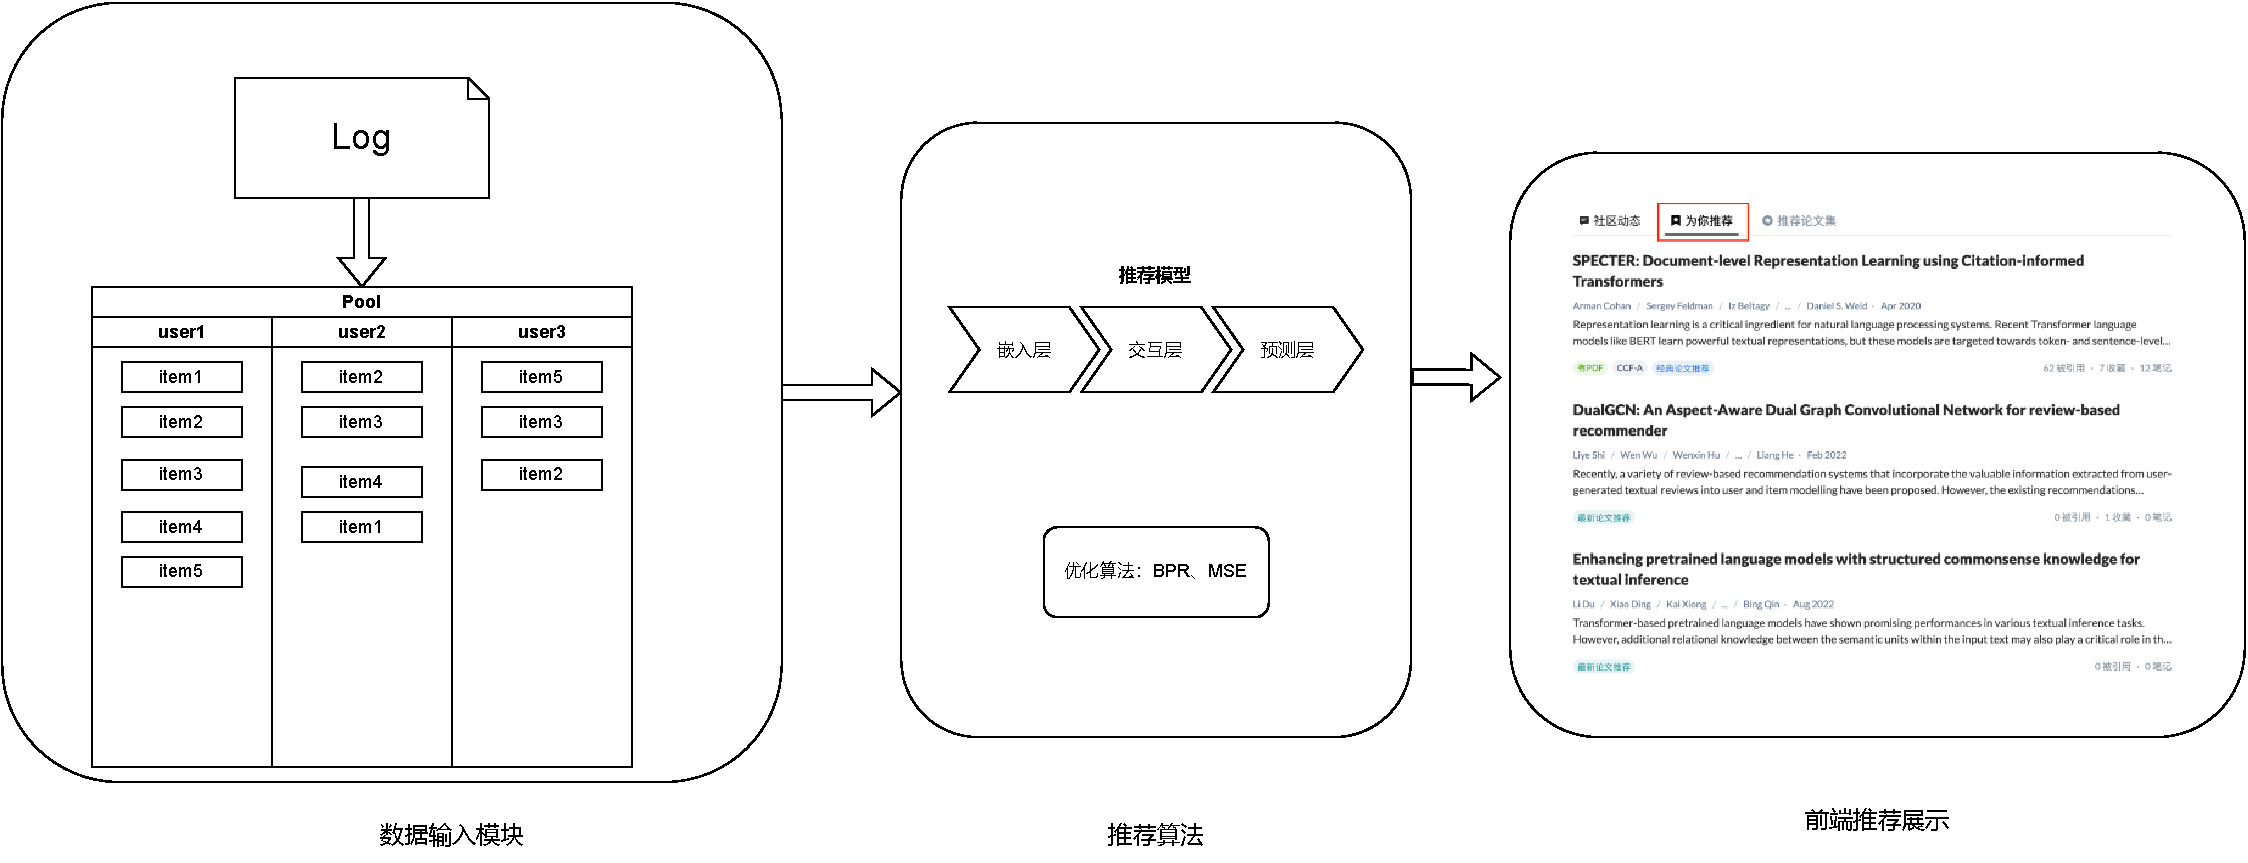
\includegraphics[width=\linewidth]{figure/rs-sys1.pdf}
%     \caption{工业推荐系统架构}
%     \label{fig:rs-systems}
% \end{figure}

\begin{figure}[!h]
    \centering
    \setlength{\belowcaptionskip}{-6mm}
    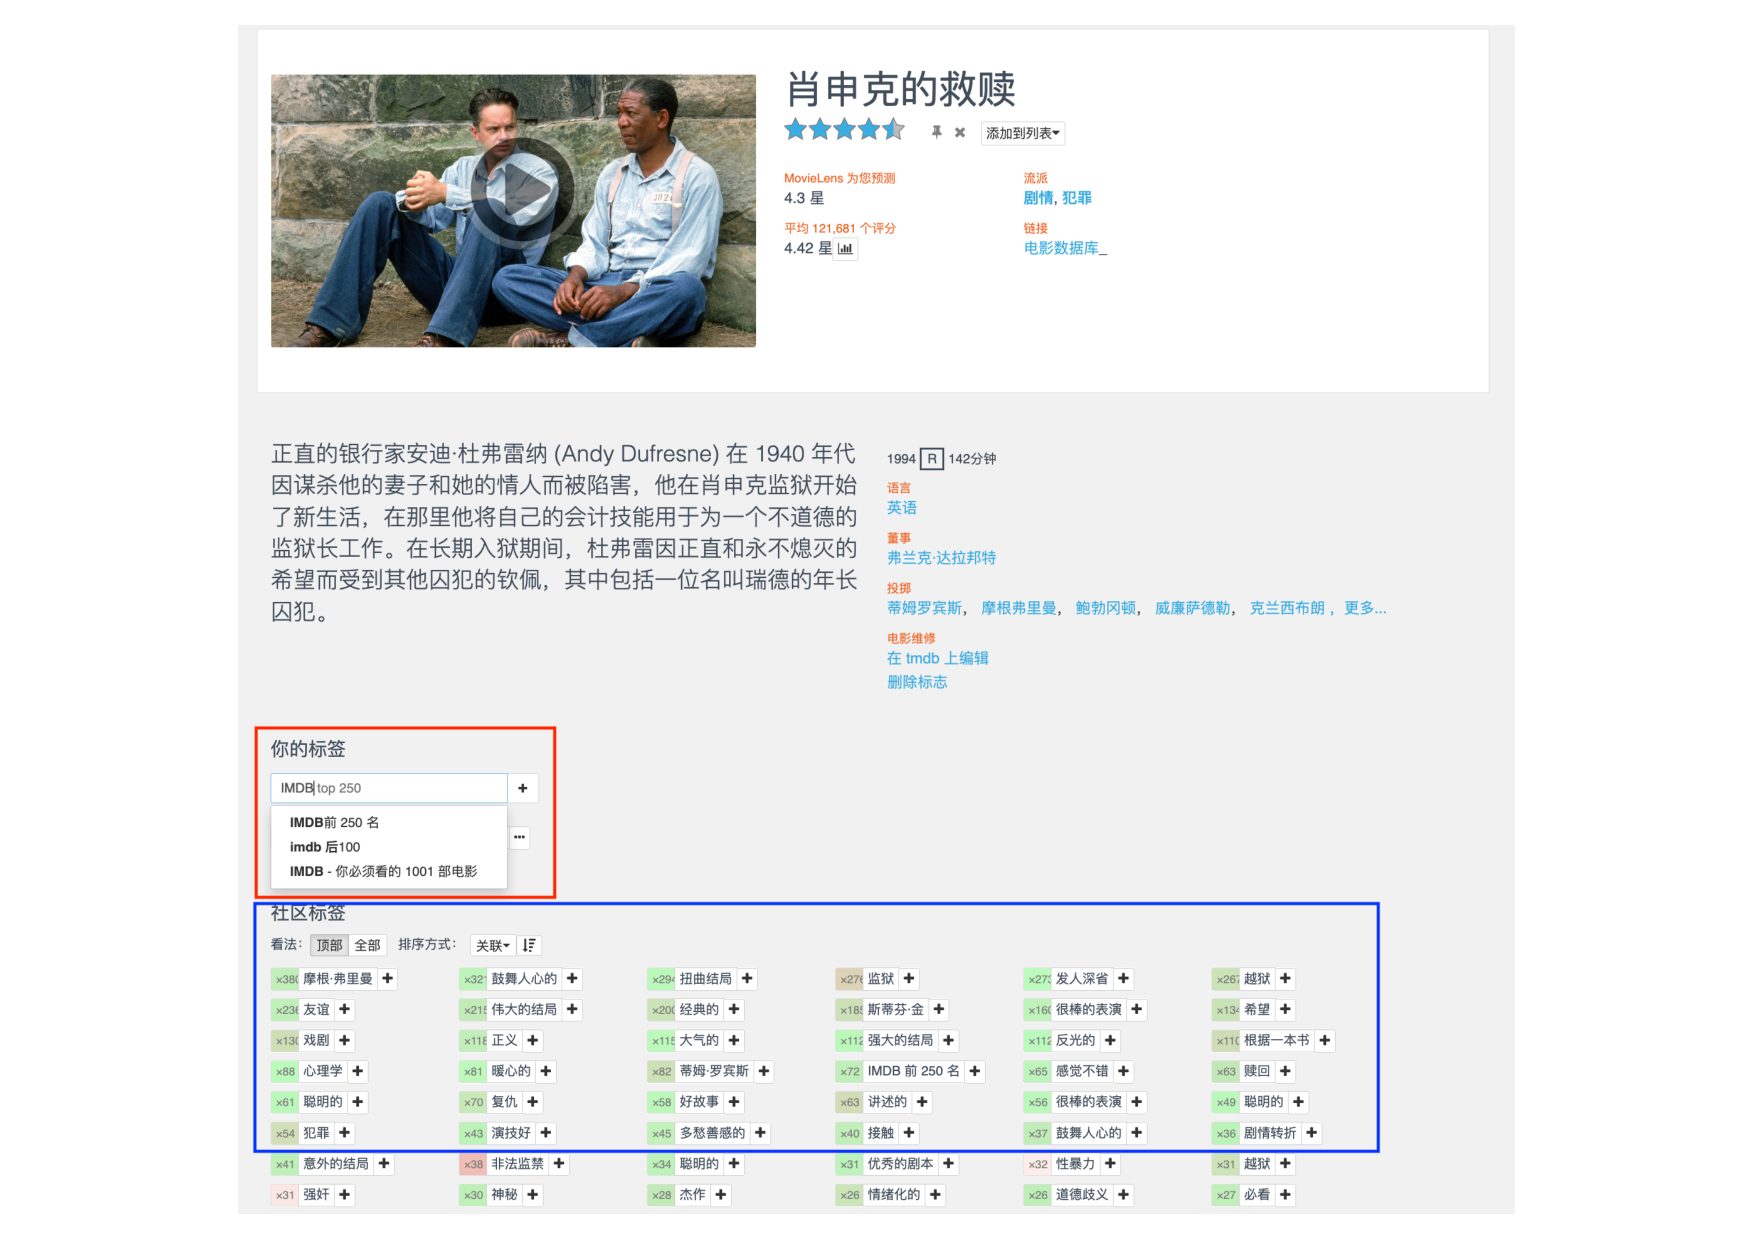
\includegraphics[width=1\linewidth]{figure/movie.pdf}
    \caption{标签感知推荐系统在电影推荐网站中的应用}
    \label{fig:movielen}
\end{figure}

在 Web 3.0 时代,用户和数据资源的关系更为丰富。用户不仅可以广泛地参与到网络互动中,并且他们所创造的数据和内容可以被下一代智能互联网归纳整理成更有价值的内容\cite{hutchison_information_2006}。许多网站提供了大众分类法(folksonomy)的功能来实现这一目标。用户可以创造并分享各种物品,同时为物品标注各种标签(tag),因此可以获得形式为 <用户,标签,物品> 的社会标签数据(folksonomy records)。如图~\ref{fig:movielen}~所示,不同的用户为电影“肖申克的救赎”标注了“越狱”或“发人深省”这样标签。内容服务平台通过积累大众标注行为(tagging behavior)为用户和物品之间构建起桥梁。这种标注行为不仅可以表达用户自身的偏好,还可以对物品内容赋予更丰富、动态的理解。因此,大众标注行为作为一种用户行为,不仅可以反映用户自身的兴趣偏好和看待物品的态度,而且物品本身蕴含的丰富内容也可以为推荐系统提供更多信息。

现有推荐系统对标签信息的应用有两类,一类是标签推荐系统(Tag Recommender Systems),其目的是在用户为物品标注标签时推荐更准确表达用户观点和需求的标签,从而构建更具规范性的标签系统,缓解不同用户知识背景带来的标签多词同义性(redundancy),或标签一词多义性(ambiguity),如图~\ref{fig:movielen} 红框中推荐的标签“IMDB top 250”。
另一类是标签感知推荐系统(Tag-aware Recommender Systems),其目的是将标签信息作为一种内容信息引入到推荐系统中,从而为用户提供个性化的物品资源推荐服务。这类应用可以运用系统内大量的大社会标注数据,有助于解决推荐系统的稀疏性和数据偏差问题。如图~\ref{fig:movielen} 蓝框中的标签,这些标签被用于推荐模型的训练,从而为用户带来更好的个性化推荐体验。

此外,由于大多数推荐方法都依赖于平台直接收集到的数据来训练模型,这将导致推荐结果继承先前模型中存在的偏见\cite{chen_bias_2021}。推荐模型倾向于将系统内流行的物品推荐给用户,因此引发了显著的流行性偏差,这使得处在长尾(long-tail)位置的物品难以被系统推荐,导致推荐系统性能下降\cite{yin_challenging_2012}。如果这样的模型被直接部署到在线服务当中,整个推荐系统将会加强数据中存在的流行性偏见问题。例如,对于电影推荐系统为例,在数据中贡献巨大的热门电影可能会被系统更为频繁的推荐,甚至对已经观看过这些电影的用户也会推荐它们。因此,推荐系统会对系统中的所有用户产生偏见,对不热门的电影产生影响,加强了系统的长尾特性。

% 2017 年,He 等人\cite{he_neural_2017}提出的神经协同过滤(Neural Collaborative Filtering,NCF)将深度学习引入到推荐系统当中,证明了深度学习可以为过去的推荐算法带来性能强大的非线性建模能力。但是,由于深度学习方法通常用于处理欧氏空间(Euclidean Space)的数据,例如图像、语音或文本,因此基于深度学习的推荐算法通常需要将各种异构数据统一到欧氏空间中\cite{wang_neural_2019}。这种处理方式丢失了数据原本存在的拓扑结构,无疑损失了可以被算法学习到的信息。在传统的推荐系统当中,用户、物品和二者之间的交互行为可以很自然的被建模成一张二部图\cite{he_lightgcn_2020};同时,现代推荐系统还将用户之间的社交网络,数据资源之间的知识图谱结合入推荐算法当中。图神经网络(Graph Neural Networks,GNN)可以捕捉节点间的关系以及整体图拓扑结构,在图的表征学习中优于传统的 PageRank、Random Walk 等算法。因此,图神经网络成为推荐算法的新研究方向\cite{kipf_semi-supervised_2017}。

当前,图神经网络、对比学习等新一代技术的涌现为解决推荐系统中存在的问题带来新的机遇。如何充分利用内涵丰富而又简洁的标签来提高推荐系统的准确性,缓解系统中的稀疏性和公平性等问题,克服上述所提到的多词同义性和一词多义性问题,已成为探索标签感知推荐系统的当务之急。

\section{研究现状及存在问题} %
本节将介绍标签感知推荐系统当前的研究现状,以及深度学习与对比学习在推荐系统中的应用。最后提出当前研究存在的问题。
\subsection{国内外研究现状}
当前,标签感知推荐系统已成为解决推荐系统中的稀疏性、公平性等问题的有效途径。该系统通过利用社会标签提供的信息,提高推荐准确性,从而增强用户对推荐结果的满意度。因此,如何充分利用标签信息来改善推荐效果成为了标签感知推荐系统的首要任务。在这一领域,研究者们提出了一系列的模型和算法。例如,Zhen 等人\cite{zhen_tagicofi_2009}提出了 TagiCofi 模型,通过利用标签信息更好地描述用户之间的相似性,从而提高协同过滤效果。为了解决标签的多词同义性问题,Shepisten 等人\citep{shepitsen_personalized_2008}提出了一种基于分层聚类的标签过滤方法,从而提升推荐性能。此外,还有一些研究在用户、物品和标签之间建立关系,以提高推荐效果。例如,Peng等人\cite{peng_collaborative_2010}提出了一种基于物品-标签对的推荐方法,而 Zhang 等人\cite{zhang_personalized_2010, zhang_solving_2012}则通过构建用户-标签-物品三部图来建模推荐系统,从而提高准确率、用户满意度和物品新颖性。除此之外,一些研究也利用标签挖掘用户和物品之间的相似性。例如,Zhao 等人\cite{zhao_folkrank_2021}提出了 FolkRank++ 模型,通过利用标签信息挖掘用户和物品之间的相似性来改善推荐效果。同时,Randle 等人\cite{rendle_learning_2009}提出了一种基于矩阵分解的推荐模型 RTF,并引入了基于个性化排名的评估方式,从而为标签感知推荐系统带来了新的发展机遇。Li等人\cite{li_tag-aware_2019}则在 Randle 等人工作的基础上提出了 BPR-T 模型,进一步完善了标签感知推荐系统的性能。

近年来,随着深度学习技术的飞速发展,越来越多基于深度学习的推荐模型应运而生。现有研究表明,采用深度学习模型能够有效提升推荐系统的性能。在深度学习模型中,主流的模型包括多层感知机(Multi-layer Perceptron, MLP)\cite{he_neural_2017,zhang_deep_2016,qu_product-based_2018,shan_deep_2016},自编码器(Autoencoder, AE)\cite{sedhain_autorec_2015, liang_variational_2018},注意力网络(Neural Attention Network, NAN)\cite{he_nais_2018, chen_attentive_2017}以及图神经网络(Graph Neural Network, GNN)\cite{wang_neural_2019,he_lightgcn_2020}等。其中,多层感知机作为一种广泛使用的深度学习模型,其强大的非线性学习能力是通过网络结构的宽度(即神经元数量)和深度(即神经网络层数)来实现的。自编码器则在多层感知机的基础上增加了额外的监督约束,引入噪声干扰来学习更为稳健的嵌入表征(embedding)。注意力网络则广泛应用于序列信息的建模场景,能够识别数据中更为重要的特征。同时,由于深度学习在图片、文章等结构性数据中的应用更为广泛,推荐系统中的用户-物品交互关系则更适合采用图建模的方式。因此,图神经网络成为了当前推荐系统领域的热门研究方向。这些深度学习模型的应用对于提高推荐系统的性能和准确性具有重要意义。

近年来,随着深度学习和图神经网络的不断发展,越来越多的推荐算法开始采用图神经网络来学习用户和物品的表示。然而,这些基于图神经网络的推荐算法通常使用传统推荐系统的优化目标函数,如基于排名的贝叶斯个性化排序(Bayesian Personalized Ranking,BPR)或均方误差(Mean Squared Error,MSE)等。具体来说,这些目标函数的训练目标和真实推荐的目标并不一致,导致训练效率低下,同时数据中的偏差问题也会被放大\cite{mao_simplex_2021,tang_multi-sample_2021}。因此,研究人员开始将对比学习引入到推荐系统中。为了解决传统推荐系统目标函数的问题,Mao 等人\cite{mao_simplex_2021}提出了一种基于余弦对比损失函数(Cosine Contrastive Loss,CCL)的推荐系统损失函数。他们将协同过滤分为交互编码器、损失函数以及负采样机制,并将余弦对比损失函数作为推荐系统损失函数进行优化,取得了出色的效果。另一方面,Hao 等人\cite{tang_multi-sample_2021}将对比学习应用于解决推荐系统中存在的样本不均衡问题,通过实验表明引入对比学习可以缓解流行性偏差等问题。除了引入对比学习外,还有其他一些方法也被用来解决推荐系统目标函数的问题。例如,一些研究者在现有的逐点型损失函数、配对型损失函数以外,引入软最大归一化损失\cite{wu_effectiveness_2022},以更准确地反映推荐系统的目标。针对传统推荐系统目标函数存在的问题,引入对比学习可以提高推荐算法的效果。未来的研究可以继续探索更有效的目标函数和学习方法来提高推荐系统的性能。

随着社交媒体和电子商务的迅猛发展,标签感知推荐系统已经成为个性化推荐研究领域的热门话题。尽管标签能够提供一些有用的信息,但由于标签数据的稀疏性,使得标签感知推荐系统在实践中面临着一些挑战。为了解决这些问题,近年来,越来越多的研究者开始探索利用深度学习技术来构建标签感知推荐系统。其中,Xu 等人\cite{xu_tag-aware_2016}提出了一种名为 DSPR 的模型,该模型使用多层感知器将用户和物品的嵌入表征映射到标签的特征空间。通过这种方式,模型可以利用神经网络的强大表征学习能力来解决标签数据的稀疏性问题。Zuo 等人\cite{zuo_tag-aware_2016}则提出了一种名为 CFA 的模型,该模型使用稀疏自编码器(Sparse Autoencoder, SAE)将用户在标签空间中的嵌入表征用于基于用户的协同过滤中。这种方法不仅可以解决标签数据的稀疏性问题,而且还可以提高推荐准确性。Chen等人\cite{chen_airec_2021}提出了一种名为 AIRec 的模型,该模型使用多层注意力网络来捕捉不同用户对于标签的偏好,从而提高推荐性能。此外,一些研究者还尝试利用图神经网络来解决标签数据中存在的多词同义性和一词多义性等问题。Huang 等人\cite{huang_tag-aware_2021}利用图神经网络对于多跳邻居语义信息的捕获能力,提出了一种高质量的个性化标签推荐模型。Chen 等人\cite{chen_tgcn_2020}在存在用户、标签、节点的异构图(heterogeneous graph)上,使用区分节点类别的消息传递机制来增强个性化推荐性能。这些基于深度学习的标签感知推荐模型为解决标签数据稀疏性问题和多词同义性、一词多义性等问题提供了有力的工具和方法,将为未来的个性化推荐系统的研究和实践带来新的思路和方向。

\subsection{现有研究存在的问题} 
目前,标签感知推荐系统中的基于深度学习的算法解决了标签空间稀疏性、一词多义和多词同义等问题,从而在推荐准确性和性能等方面展现出了优越性。然而,现有的研究方法也存在着一些问题,这些问题限制了模型性能的提升。

(1)现有的标签感知推荐系统涉及到的交互类型繁多,如何高效组织数据,并进一步建模数据中的多种交互类型极具挑战。在标签感知推荐系统中,有一些模型将标签作为用户的特征进行编码\cite{zuo_tag-aware_2016,chen_airec_2021},而另一些模型将标签作为与用户、物品同级的实体进行建模\cite{zhang_personalized_2010,chen_tgcn_2020}。然而,这些建模方法在直接应用于图神经网络的模型时,会进一步放大数据的稀疏性,因此需要进行进一步的调整;

(2)现有应用图神经网络的模型仅仅使用了原始神经网络的设定,而没有根据标签感知推荐系统进行进一步调整。有些模型使用了复杂的消息传播机制\cite{wang_neural_2019,chen_tgcn_2020},这使得模型的训练难度大幅增加,需要更多的训练轮数才能使得模型收敛。相比之下,简单的消息传播机制不仅有效降低了训练难度,还通过多跳邻居提供了丰富的上下文语义,从而有效地缓解了一词多义和多词同义问题;

(3)现有模型所采用的优化机制往往忽略了图神经网络自身的特点,盲目地沿用传统推荐算法的优化目标进行模型优化。大多数模型仅仅使用 BPR 单一损失作为优化方向,忽略了现代推荐系统中广泛存在的流行性偏差问题。在多任务学习的设定下,联合使用知识图谱、对比学习等方法可以有效地克服数据中存在的偏见,使得推荐系统得到的结果更为公平。

\section{研究内容与贡献} %
本节将介绍本文的主要研究内容,介绍研究该课题的必要性。同时总结本文成果,概括本文对于该领域的学术贡献。
\subsection{本文研究内容} % 为什么要做这个研究
本文旨在将标签信息融入推荐算法,以构建用户和物品的桥梁。针对标签感知推荐系统目前面临的问题,本文将深入探讨社会标签信息中存在的图数据结构,为用户-标签-物品的交互过程做出合理的建模。同时,将利用图神经网络和对比学习,提出两种标签感知推荐模型,最终为用户带来优秀的 Top-K 个性化推荐能力。本文的研究内容主要包括以下四个方面:

(1) 深入探索标签感知推荐系统

本文将标签感知推荐系统的研究重点划分为数据与算法两个部分。对于社会标注数据部分,本文分析过去文献对数据的建模方式存在的问题,为用户-标签-物品的交互过程做出合理的建模。同时,对于标签感知推荐算法,本文将标签感知推荐系统抽象为数学形式,为后续研究打下基础。

(2) 提出基于图神经网络的标签感知推荐模型

为避免图神经网络中冗余的架构,本文去除了不适用于标签感知推荐系统的部分,提出了轻量化设计的图神经网络算法。该模型主要由轻量化设计的图神经网络结构组成。此外,本文利用基于知识图谱的标签关系映射的正则化函数为该模型学习到更稳健的特征。

(3) 提出基于对比学习的标签感知推荐模型

为避免在数据中广泛存在的推荐系统不公平现象,本文提出了基于图对比学习的标签感知推荐系统。在轻量化图神经网络算法的基础上,使用带有知识图谱与对比学习的多任务优化任务进行模型优化。

(4)实验验证和结果分析

本文提出的两个模型在三个公开数据集上与标签感知推荐系统领域主流模型进行对比。实验结果表明,本文提出的模型具有优越的 Top-K 推荐性能。同时,本文还在一个真实运行的系统数据中验证了模型的有效性。

\subsection{研究贡献} % 功能 原理()我具体做了什么研究

本文主要探讨了推荐系统中的标签感知问题以及不公平现象,通过重新设计的社会标注图(Folksonomy Graph,FG)的基础上,提出了轻量化社会标注图协同过滤(Light Folksonomy Graph Collaborative Filtering, LFGCF)和标签图对比学习框架(Tag-aware Graph Contrastive Learning,TAGCL)

(1)本文首先提出了一种新的社会标注图,该图由用户-标签图和物品-标签图组成,降低了异构图的复杂度,方便后续模型的设计和优化;

(2)本文基于图神经网络,提出了一种轻量化的标签感知推荐模型 LFGCF。为了适应推荐系统的特性,该模型去除了图卷积神经网络的特征变换和非线性激活组件,并采用加权和聚合函数进行消息传播,从而提高了模型推荐的精准度,并降低了模型的训练难度;

(3)本文探讨了推荐系统中存在的不公平现象,提出了一种新的模型 TAGCL。该模型使用对比学习和知识图谱联合优化模型,在训练过程中对标签进行同时采样,从而有效地提高了模型推荐的精准度和公平性;

(4)本文设计了一系列实验以评估 LFGCF 和 TAGCL 的性能,并与当前主流的推荐算法模型进行对比。本文还在一个真实运行的系统数据中验证了提出模型的有效性。

综合来看,本文的研究贡献为标签感知推荐系统和数据中的不公平问题提供了新的思路和解决方案。

\section{本文创新点} % 功能 原理()我具体做了什么研究

本文的主要创新点有以下三点:

(1)本文提出一种新的社会标注图结构。该图分别由用户-标签图和物品-标签图组成,创新性地降低了异构图的复杂度;

(2)本文提出了基于轻量化图神经网络的推荐模型 LFGCF。本文去除图卷积神经网络的特征变换与非线性激活组件,并使用加权和聚合函数进行消息传播。创新性的轻量化设计降低了模型的训练难度,并提高了模型推荐的精准度;

(3)本文提出了基于对比学习的推荐模型 TAGCL。在模型优化时,使用对比学习与知识图谱联合优化模型,在训练过程中对标签进行同时采样。创新性地应用了多任务学习框架,提高模型推荐精准度的同时优化了推荐系统中不公平的现象。

\section{本文组织架构}
本论文分为 6 章进行组织,第~\ref{cha:introduce}~引言介绍标签感知推荐的研究背景和研究意义,并阐述本文的主要研究内容与创新点。第~\ref{cha:tagrec}~章介绍社会标签数据和标签感知推荐系统的定义。第~\ref{cha:lfgcf}~介绍基于轻量化图神经网络的推荐算法研究工作。第~\ref{cha:tagcl}~章介绍基于对比学习的推荐算法研究工作。第~\ref{cha:ex_demo}~章介绍推荐算法实验结果与数据分析。最后在第~\ref{cha:end}~章总结全文,具体安排如下:
\begin{figure}[!h]
    \centering
    \setlength{\belowcaptionskip}{-6mm}
    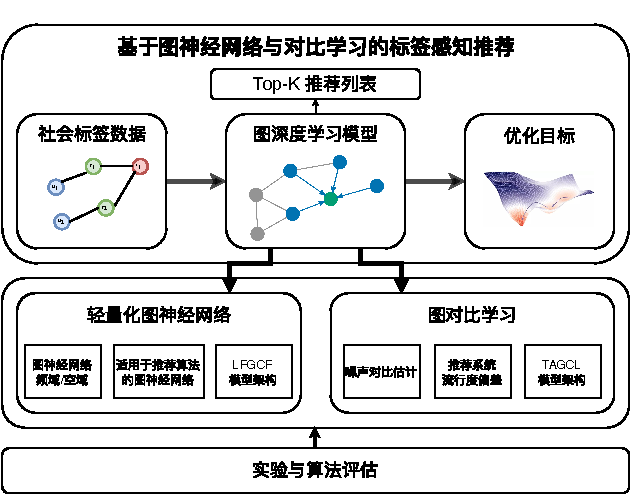
\includegraphics[width=0.7\linewidth]{figure/structure.drawio.pdf}
    \caption{本文组织架构}
    \label{fig:structure}
\end{figure}

第~\ref{cha:introduce}~章介绍了标签感知推荐系统的背景和研究意义,并总结了国内外研究现状及其存在的问题。同时概括了本文的研究内容、贡献和创新点,并提出了本文的架构。

第~\ref{cha:tagrec}~章首先综述了基于深度学习、图神经网络和对比学习的推荐算法的相关研究。接着深入探讨了现有研究存在的问题,并阐述了本文的技术路线。对研究中所涉及的图神经网络、对比学习和推荐系统的公平性等理论和技术进行了介绍。最后,构建了本文的核心建模——社会标注图,并定义了标签感知推荐系统的数学形式。

第~\ref{cha:lfgcf}~章首先详细地介绍了图神经网络,并且介绍了图神经网络应用与推荐算法的两个模型。之后详细介绍了本文提出的基于轻量化图卷积网络的 LFGCF。特别是如何去除原始图神经网络中不必要的组件,从而构建轻量化的图神经网络模块,从消息传播层、卷积层合并和模型输出角度介绍模型,并介绍了模型的训练细节。

第~\ref{cha:tagcl}~章首先介绍了对比学习并推导了对比学习中最重要的损失函数 InfoNCE。之后详细介绍本文提出的基于轻量化图卷积网络的 TAGCL,着重描述如何利用对比学习以及副标签采样和 TransT 解决数据中的流行度偏差,并介绍了 TAGCL 的训练细节。

第~\ref{cha:ex_demo}~章主要对本文提出的两个模型 LFGCF 和 TAGCL 进行实验验证和性能分析。首先简要介绍了实验使用的数据集、数据预处理方法、实验流程、评估指标和对比模型,然后阐述了实验模型相关参数配置。评估结果表明,与现有标签感知推荐模型相比,本文提出的解决方案具有显著的性能提升。此外,设计了多组实验对模型的结构和相关参数进行评估。最后,本文在一个真实运行的推荐系统数据中进行离线实验,结果表明模型可以有效的提高推荐性能。

第~\ref{cha:end}~章对本文的研究工作进行简要总结,并对下一阶段的工作进行展望,为后续标签感知推荐模型的研究指明方向。

